\newcommand{\Constraints}[1]{\mathsf{constraints}({#1})}
\newcommand{\Frac}[1]{\mathsf{frac}({#1})}
\newcommand{\Addtimer}[4]{\mathsf{addtimer}({#1,#2,#3,#4})}

\section{From timed to untimed learning}  
\label{algorithm}
In this section, we consider another instance of Angluin's MAT framework.
Again, the teacher knows an MMT $\M$ but now the learner poses membership queries
to learn the \emph{untimed} behaviors of $\M$, and if an equivalence query fails then the counterexample is an \emph{untimed} behavior of $\M$.
We will show how an untimed teacher for MMTs can be implemented using a timed teacher.

\subsection{An untimed MAT framework for MMTs}
\label{sec:untimed-mat}
Given the equivalence of the timed and the untimed semantics of MMTs, it is natural to also 
consider an untimed setting, in which a learner tries to construct an MMT based on membership queries for untimed behaviors.

\todofv{Move canonical forms to section on untimed semantics?}
In the untimed framework, the teacher does not reveal the names of the timers of $\M$. 
It brings untimed behaviors into a ``canonical'' form, so that a learner can only observe these behaviors up to isomorphism.
Let us formalize this idea.
Suppose $\beta$ be an untimed behavior in which transitions update at most one timer.
We say that $\beta$ is in \emph{canonical form} if, for each $j$, the timer that is updated in the $j$-th event
(if any) is equal to $x_j$.
For each untimed behavior $\beta$ in which transitions update at most one timer, there is a unique untimed behavior
$\beta'$ in canonical form that is isomorphic to $\beta$.
We write $\can{\beta}$ to denote this $\beta'$.
\todofv{Add example}

Consider an untimed behavior $\beta$ in canonical form:
\begin{eqnarray*}
\beta & = & X_0 \xrightarrow{i_1/o_1, \rho_1} X_1  \cdots \xrightarrow{i_k/o_k, \rho_k} X_{k}.
\end{eqnarray*}
Let $1 \leq l \leq j \leq k$, $d \in \natplus$ and suppose that 
(1) $\rho_l$ either starts no timer or sets $x_l$ to $d$,
(2) $\beta$ does not contain a timeout event $\toevent{x_l}$.
Then $\Addtimer{l}{d}{j}{\beta}$ is the untimed behavior obtained from $\beta$ by
replacing $\rho_l$ by the update $x_l := d$, and adding $x_j$ to the sets $X_l$ up to (and including) $X_j$.
%In the untimed behavior $\emptyset \xrightarrow{i/o,~ x:=1 } \{ x\} \xrightarrow{i/o,~ y:=60 } \{ x, y\}$, for instance, we may remove timer $x$
%and obtain $\emptyset \xrightarrow{i/o } \emptyset \xrightarrow{i/o,~ y:=60 } \{ y\}$.
%Similarly, we may remove the first use of timer $x$ in the untimed behavior 
%$\emptyset \xrightarrow{i/o,~ x:=1 } \{ x\} \xrightarrow{i/o,~ x:=5 } \{ x\} \xrightarrow{\toevent{x}/o} \emptyset$ and obtain
%$\emptyset \xrightarrow{i/o } \emptyset \xrightarrow{i/o,~ x:=5 } \{ x\} \xrightarrow{\toevent{x}/o} \emptyset$.
Write $\beta \sqsubseteq \beta'$ if $\beta'$ can be obtained from $\beta$ by zero or more applications of function $\mathsf{addtimer}$.
Observe that $\sqsubseteq$ is a partial order with as minimal elements untimed behaviors in which every timer that is started also times out.
We call such untimed behaviors \emph{lean}.
We say that $\beta$ is a \emph{partial} untimed behavior of MMT $\M$ iff $\M$ has an untimed behavior $\beta'$ such that $\beta \sqsubseteq \beta'$.
\todofv{Add example}
%In the untimed framework, the teacher replies with partial untimed behaviors of $M$, brought in canonical form.

An \emph{untimed input word} over $I$ is a sequence $u = i_1 \cdots i_k$ over $\extinputs$ such that (1)
for all indices $j, l$, $i_j = \toevent{x_l}$ implies $l < j$, and (2) each timer occurs at most once in a timeout event.
The first condition  says that if a timer expires it must have been set in a previous event, and the second condition  expresses that
each timer may expire at most once.
Let $\beta$ be an untimed behavior in canonical form.
We can associate a unique input word $\untimedinputword(\beta)$ to $\beta$ by removing all the output events,
updates, and timer sets from $\beta$.
\todofv{Add example}
\iflong
\begin{figure}
\begin{center}
 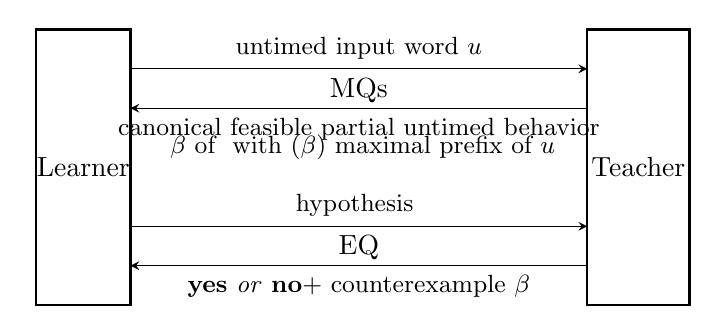
\begin{tikzpicture}[>=stealth]
            \draw [thick] (0,0) rectangle (1.2,3.5) node[midway] {Learner};
            \draw [thick] (7,0) rectangle (8.3,3.5) node[midway] {Teacher};
            \draw [->] (1.2,3) -- (7,3) node[midway,below] {MQs};
            \draw (1.2,3) -- (7,3) node[midway,above] {\small untimed input word $u$};
            \draw [<-] (1.2,2.5) -- (7,2.5) node[midway,below] {\small canonical feasible partial untimed behavior};
             \draw (4.15,2) node {\small $\beta$ of $\M$ with $\untimedinputword(\beta)$ maximal prefix of $u$};
            \draw [->] (1.2,1) -- (7,1) node[midway,below] {EQ};
            \draw (1.2,1) -- (7,1) node[midway,above] {\small hypothesis $\CH$};
            \draw [<-] (1.2,0.5) -- (7,0.5) node[midway,below] {\small {\bf yes} \emph{or} {\bf no}+ counterexample $\beta$};
        \end{tikzpicture}
\end{center}    
\caption{Untimed MAT framework}
\label{fig:untimed MAT}
\end{figure}
\fi

Our untimed learning setup
\iflong
, illustrated in Figure~\ref{fig:untimed MAT}, 
\fi
is similar to the timed setup:
again the teacher knows an MMT $\M$ and the learner initially only knows the set of inputs $I$ of $\M$.
Again, the learer may pose membership and equivalence queries.
But now a \emph{membership query} consists of an untimed input word $u$ over $I$.
The teacher replies with a maximal feasible partial untimed behavior $\beta$ of $M$ (in canonical form) such that
$\untimedinputword(\beta)$ is a prefix of $u$.
With an \emph{equivalence query}, the learner asks if a hypothesis $\CH$ with inputs $I$ is correct.
Upon receiving $\CH$, the teacher answers \emph{yes} if $\CH \approx_{\mathit{untimed}} \M$.
Otherwise it answers \emph{no} and supplies a counterexample, which now is a feasible untimed behavior $\beta$ (in canonical form) that
is a partial untimed behavior of $\M$ but not of $\CH$ (by Lemma~\ref{not untimed} such a counterexample exists).

\subsection{Zones and constraints}

In order to implement an untimed teacher using a timed teacher, we need a
basic machinery to determine whether an untimed behavior is feasible, i.e.,
whether it can be derived from a timed word. This can be done using
well-established techniques for manipulating difference-bound matrices
(DBMs) that are in standard use for analyzing timed
automata~\cite{Di89,BengtssonY03}.
In this section, we describe an adaptation of such techniques to
our setting.

Let $\beta$ be an untimed behavior in canonical form:
\begin{eqnarray*}
\beta & = & \emptyset \uttrans{i_1}{o_1}{\rho_1} X_1  \cdots X_{k-1} \uttrans{i_k}{o_k}{\rho_k} X_k.
\end{eqnarray*}
We would like to determine for which values $d_1, \ldots , d_{k+1}$
a corresponding timed behavior
\[
\tvals_0 \dtrans{d_1} \tvals'_0 \uttrans{i_1}{o_1}{\rho_1}
\quad \cdots \quad
\dtrans{d_k} \tvals'_k \uttrans{i_k}{o_k}{\rho_k} \tvals_k
\dtrans{d_{k+1}} \tvals'_{k+1}
%% \uttrans{\toevent{x_i}}{o_{n+1}}{\rho_n}
\]
is possible. We solve this problem by producing a constraint over the
values $d_1, \ldots , d_{k+1}$. In order to use DBM techniques, we first
change representation by letting
$t_j = d_1 + \cdots + d_j$ for $j = 1 , \ldots, k+1$. Intuitively, $t_j$ is
the time of occurrence of the $j$th transition in $\beta$.
We now associate with $\beta$ a conjunction of difference constraints over
$t_1, \ldots, t_{k+1}$, denoted $\Constraints{\beta}$, consisting of
%\todobj{We assume that delays are always non-zero. Check how this is said in the paper}
\begin{itemize}
%% \item
%% $0 < t_1 \leq d_{\max}$,
%% \item
%% for each index $j < k$:  $0 <  t_{j+1} - t_j \leq d_{\max}$,
\item
for each index $j$ with $1 \leq j \leq k$:  $0 <  t_{j+1} - t_j$,
\item
for each timeout event $i_j = \toevent{x_l}$: $t_j - t_l = \rho_l(x_l)$,
\item
for each clock $x_l$ that is started but does not timeout: $t_j -t_l < \rho_l(x_l)$,
where $j$ is the largest index such that $x_l \in X_j$,
%% \item
%% for each pair of distinct indices $j$ and $l$ with $i_j, i_l \in I$: $\Frac{t_j} \neq \Frac{t_l}$ 
%% (to express that the fractional parts of $t_j$ and $t_l$ are different).
\end{itemize}
By standard DBM techniques, we can check whether $\Constraints{\beta}$ is satisfiable by saturating it (i.e., closing it under implied constraints, which
will always be of form
$n < t_j - t_l < m$ or $t_j - t_l = m$ for integers $n,m$), and checking that
all such differences allow $t_{j+1} - t_j$ be positive for each $j$.
We infer that $\beta$ is feasible iff $\Constraints{\beta}$ is satisfiable.
Moreover, if $\beta$ is feasible, we can use the techniques of
Section~\ref{sec:wiggling} to construt a solution
such that $\Frac{t_j} \neq \Frac{t_l}$ for each pair of distinct indices $j$ and $l$ with $i_j, i_l \in I$.

From the saturated version of $\Constraints{\beta}$, we also derive a constraint,
denoted $\Zone{\beta}$,
which characterizes the possible timer valuations $\tvals_k$ in a timed
behavior of the above form.  The constraint $\Zone{\beta}$
contains for each pair of timers $x_i,x_j$ in $X_k$ the conjunct
\[
(m + \rho_j(x_j) - \rho_i(x_i)) < \tvals_k(x_j) -\tvals_k(x_i) < (n + \rho_j(x_j) - \rho_i(x_i))
\]
whenever the saturated version of $\Constraints{\beta}$ contains the conjunct
\(
m < t_j - t_i < n
\).
(This can be derived using
$\tvals_k(x_j) = \rho_j(x_j) - (t_k - t_j)$
and
$\tvals_k(x_i) = \rho_i(x_i) - (t_k - t_i)$).

\iflong
We can derive the following lemmas.

\begin{lemma}
\label{lemma: feasibility concatenation}
Suppose $\beta, \beta'$ are untimed behaviors such that
$\Zone{\beta} = \Zone{\beta'}$. Let $\gamma$ be any untimed behavior.
Then $\beta \cdot \gamma$ is feasible iff $\beta' \cdot \gamma$ is feasible.
\end{lemma}

\begin{lemma}
\label{lemma finitely many zones}
$\{ \Zone{\beta} \mid \beta \mbox{ feasible untimed behavior of } \M \}$ is finite.
\end{lemma}
\fi
%% \ifshort
%% \begin{proof}
%% See appendix.
%% \end{proof}
%% \else
%% \begin{proof}
%%   An MMT only has a finite number of timers that can only be set to a finite number of integer values. Since in an MMT the values of timers can only decrease, their values are bounded, so that only finitely many integers may appear in the conjuncts of $\Zone{\beta}$. This the set of possible $\Zone{\beta}$ is finite.
%% \end{proof}
%% \fi

Let $\beta$ be a feasible untimed behavior and let $x \in X$ be a timer. Then we say that $x$ is \emph{expirable} after $\beta$
if there exists a valuation in $\Zone{\beta}$ in which $x$ is minimal.

\begin{lemma}
\label{expirable}
Suppose $\beta$ is a feasible untimed behavior with $\Last{\beta} = Y$ and $Y \uttrans{\toevent{x}}{o}{\rho} Y'$ is an untimed behavior.
Then $x$ is expirable after $\beta$ iff $\beta \uttrans{\toevent{x}}{o}{\rho} Y'$ is feasible.
\end{lemma}


%Note that for an untimed behavior $\beta$, the set $\zone{\beta}$ of valuations that can be reached with a timed behavior $\sigma$ with %$\untime(\sigma) = \beta$ can be symbolically represented using DBMs \cite{Di89}.
%We can do this since the transition relations $\xrightarrow{d}$ and $\xrightarrow{i_1/o_1, \rho_1}$ can be decomposed 
%into elementary operations on DBMs such as reset, conjunction, and delay successors \cite{BengtssonY03}.
%This allows us to compute whether an untimed behavior $\beta$ is feasible ($\zone{\beta}$ is empty), and
%whether a timer $x$ may expire after $\beta$ ($\zone{\beta}$ contains a valuation in which $x$ is minimal).

\subsection{Building an untimed from a timed teacher}
We will now show how to construct an adapter that transforms a teacher for the timed setting into a teacher for the untimed setting.
The adapter maintains an integer variable $d_{\max}$ to store an estimate of the maximal timeout value that occurs in $\M$. Initially, the
adapter sets $d_{\max}$ to an arbitrary value, which may be increased based on the (transparent) timed words that it receives from
the timed teacher.

Suppose the untimed teacher receives a membership query, consisting of an untimed input word $u = i_1 \cdots i_k$.
We present an algorithm that constructs a response for $u$, that is, a feasible partial untimed behavior 
$\beta$ of $\M$ in canonical form with $\untimedinputword(\beta)$ a maximal prefix of $u$.
The algorithm maintains a variable $B$ that stores the fragment of $\beta$ computed thus far, and a counter $j$ that ranges from $0$ to $k$.
Initially $B$ is set to the trivial untimed behavior $\emptyset$ and $j$ to $1$.
The algorithm then enters its main loop in which the following case statement is performed while $j \leq k$.  
We will maintain as a loop invariant that $B$ is a feasible untimed behavior with $j-1$ inputs.
\begin{enumerate}
\item
Case $i_j \in I$. Let $N := B ~ i_j/\omega/\rho_0 ~ \emptyset$, where $\omega \in O$ is an arbitrary output that acts as placeholder
and $\rho_0$ is the empty update. (We omit the arrow for $i_j/\omega/\rho_0$ here.)
Since $B$ is feasible (by the loop invariant), it follows by Lemma~\ref{feasible plus input is feasible} that
extension $N$ is also feasible.
Thus the constraints in $\Constraints{N}$ are satisfiable and we may compute a solution $t_1 ,\ldots, t_j$.
Let $t_0 = 0$, $d_j = t_j - t_{j-1}$, for $j = 1,\ldots, j$, and let
$o_1 ,\ldots, o_{j-1}$ be the output events occurring in $B$. 
Then $w = d_1 ~ i_1 ~ o_1 ~ d_2 ~ i_2 ~ o_2 \cdots d_j ~ i_j ~ \omega$ is a transparent timed word.
Let $u' = \timedinputword(w)$ be the corresponding transparent timed input word.
Forward membership query $u'$ to the timed teacher, and
let $w'$ be the response.
If $w'$ and $w$ are equal, except possibly for the last output symbol, which is $o_j$ in $w'$,
then we set  $B := B ~ i_j/o_j/\rho_0 ~ \emptyset$, increment counter $j$, and finish the body of the loop.
Otherwise, $w'$ contains some timeout event that was not supposed to happen according to untimed input word $u$.
Since $u'$ is transparent, $w'$ is transparent as well. 
Thus we may extract from $w'$ which event $l$ started the timer, to which value
$e$ the timer was set, and the index $m$ of the timeout event.
We set $B := \Addtimer{l}{e}{m-1}{B}$ and finish the body of the loop. 
\item
Case $i_j = \toevent{x_l}$, for $l < j$.
If timer $x_l$ is started in $B$ and initialized with the value $e$ then
let $N := \Addtimer{l}{e}{j-1}{B} ~ \toevent{x_l}/\omega/\rho_0 ~ \emptyset$.
Check whether $\Constraints{N}$ is satisfiable. If so proceed to (*), otherwise exit the while loop.
If timer $x_l$ is not started in $B$, let
$N^e = \Addtimer{l}{e}{j-1}{B} ~ \toevent{x_l}/\omega/\rho_0 ~ \emptyset$, for $e = 1 ,\ldots, d_{\max}$.
If there exists an $e$ for which $\Constraints{N^e}$ is satisfiable, set $N := N^e$ and proceed to (*),
otherwise exit the while loop.

\vspace{0.3em}
(*) Compute a solution $t_1 ,\ldots, t_j$ for $\Constraints{N}$.
Let $t_0 = 0$, $d_j = t_j - t_{j-1}$, for $j = 1,\ldots, j$, and let
$o_1 ,\ldots, o_{j-1}$ be the outputs occurring in $B$. 
Then $w = d_1 ~ i_1 ~ o_1 ~ d_2 ~ i_2 ~ o_2 \cdots d_j ~ \toevent{x_l} ~ \omega$ is a transparent timed word.
Let $u' = \timedinputword(w)$ be the corresponding transparent timed input word.
Forward membership query $u'$ to the timed teacher, and let $w'$ be the response.
Since $u'$ is transparent, $w'$ is transparent as well.
If $w'$ and $w$ are equal, except possibly for the last output symbol, which is $o_j$ in $w'$,
set $B$ equal to $N$ with the last output changed to $o_j$, increment counter $j$, and finish the body of the while loop.
It may also occur that, even though the last event of $w'$ is a timeout triggered by event $i_l$, the value $e'$ to which this timer is
set is different from $e$. In this case  set
$B := \Addtimer{l}{e'}{j-1}{B} ~ \toevent{x_l}/o_j/\rho_0 ~ \emptyset$, where $o_j$ is the last output in $w'$,
increment counter $j$ and finish the body of the while loop.
Finally, it may occur that $w'$ contains some timeout event that was not supposed to happen according to untimed input word $u$.
In this case, we extract from $w'$ which event $l$ started the timer, to which value
$d$ the timer was set, and the index $m$ of the timeout event.
Set $B := \Addtimer{l}{d}{m-1}{B}$ and finish the body of the while loop. 
\end{enumerate}
After termination of the while loop, the algorithm returns the feasible untimed behavior $B$.
Note that the number of iterations of the main loop is linear in the size of $u$.
\todofv{Add example!}
%\paragraph{Example}
%Consider a scenario where the timed teacher knows the MMT of Figure~\ref{fig:nondeterminism} (bottom).
%Suppose that $d_{\max} = 5$ and the untimed teacher receives a query for input word $i ~ i$. The adapter starts with defining
%\[
%\beta_0 = \emptyset
%\]
%Next it solves $\Constraints{\emptyset ~ i ~ \omega ~ \emptyset} = \{ 0 < t_1 \leq 5 \}$.
%Suppose it arrives at the solution $t_1 = 1$. Based on this, the timed input word $1 ~ i ~ 0$ is
%forwarded to the timed teacher. The timed teacher responds with $1 ~ i ~ o$ and the adapter defines
%\[
%\beta_1 = \emptyset ~ i ~ o ~ \emptyset
%\]
%The constraints in $\Constraints{\emptyset ~ i ~ o ~ \emptyset ~ i ~ \omega ~ \emptyset}$ are still trivial.
%Suppose adapter finds solution $t_1 = 1,~ t_2 = 4.1$ and forwards timed input word  $1 ~ i ~ 3.1 ~ i ~ 0$ to the timed teacher.
%Based on the response $1 ~ i ~ o ~ 2 ~ \mathit{to} ~ o$, the adapter realized that the first transition starts a timer
%and solves $\Constraints{\emptyset ~ i,x:=1 ~ o ~ \{ x \} ~ i ~ \omega ~ \emptyset}$.

Implementing equivalence queries is easy.
Suppose that the untimed teacher receives an equivalence query $\CH$.
Then we just forward this query to the timed teacher.
If the timed teacher answers \emph{yes} then $\CH \approx_{\mathit{timed}} \M$.
In this case, by Theorem~\ref{timedimpliesuntimed}, $\CH \approx_{\mathit{untimed}} \M$,
and thus the untimed teacher should also return the result \emph{yes}.
If the timed teacher answers \emph{no} and returns a counterexample $w$,
then $w$ is a transparent timed word of $\M$ but not of $\CH$.
In this case, by Theorem~\ref{untimedimpliestimed}, we may conclude that
$\CH \not\approx_{\mathit{untimed}} \M$, and thus the untimed teacher should also return a result \emph{no}.
Since $w$ is a transparent timed word of $\M$, it 
follows 
\iflong
by Lemma~\ref{lemma unique causality map} 
\fi
that $w$ 
has a unique causality map $c$.
This allows us to transform $w$ into a feasible untimed behavior $\beta$ in canonical form that is a partial untimed
behavior of $\M$ but not of $\CH$: the causality map tells us exactly which timers are set and timeout. 
Thus the untimed teacher may return $\beta$ as counterexample.
If our estimate $d_{\max}$ of the maximal timeout value of $\M$ is too low, then it may occur that in $w$ the timeout value of some
timer is larger than $d_{\max}$. In this case, the value of $d_{\max}$ is updated to the newly observed maximal timeout value.
\todofv{Think through implications of updating $d_{\max}$.}





